\subsection{Předzpracování datasetů}
\label{subsec:predzpracovani_datasetu}
Z datasetů byly extrahovány potřebné biosignály, které byly následně zpracovány
a normalizovány na úrovní subjektů. Metodika zpracování vychází ze
sekce~\ref{sec:zpracovani_biosignalu}. Normalizace byla provedena škálováním
biosignálů tak, aby měly průměrnou hodnotu nula a směrodatnou odchylku jedna. To
bylo dosaženo odečtením střední hodnoty biosignálu od každé jeho hodnoty a
následným vydělením směrodatnou odchylkou.

Vzhledem k tomu, že dataset CLAS neobsahuje signál RSP, byl tento signál
vytvořen pomocí metody \gls{EDR} (ECG-Derived Respiration). Jedná se o extrakci
informace o dýchání z elektrokardiogramu. Knihovna \textit{Neurokit2} poskytuje
implementaci algoritmu podle~\cite{VanGent2019}, jež byla pro tyto účely
použita.

Následně byly všechny signály segmentovány na 5s, 5s s 50\% překryvem a 1s
úseky. Z těchto segmentů byly poté vytvořeny příznaky pro účely strojového
učení. Blíže je tvorba těchto příznaků a jejich využití popsáno v
sekci~\ref{sec:hybridni_detekce}. Byly ponechány pouze ty segmenty, které svojí
třídou korespondovaly žádanému kognitivnímu stavu.

\begin{figure}[h]
    \centering
    \framebox[\textwidth]{%
        \begin{subfigure}[b]{0.45\textwidth}
            \dirtree{%
                .1 Datasets.
                .2 WESAD.
                .3 S2.
                .4 S2.pkl.
                .4 $\vdots$.
                .3 S3.
                .3 $\vdots$.
                .2 CLAS.
                .3 Part1.
                .4 full\_ecg.csv.
                .4 full\_gsr\_ppg.csv.
                .4 $\vdots$.
                .3 Part2.
                .3 $\vdots$.
            }
            \caption{Původní struktura datasetů}
            \label{subfig:tree1}
        \end{subfigure}
        \hfill
        \begin{subfigure}[b]{0.45\textwidth}
            \dirtree{%
                .1 Datasets.
                .2 WESAD.
                .3 merged\_1s.pkl.
                .3 merged\_5s.pkl.
                .3 merged\_5s\_2s.pkl.
                .3 $\vdots$.
                .2 CLAS.
                .3 merged\_1s.pkl.
                .3 merged\_5s.pkl.
                .3 merged\_5s\_2s.pkl.
                .3 $\vdots$.
            }
            \caption{Zpracované datasety}
            \label{subfig:tree2}
        \end{subfigure}
    }
    \caption{Porovnání struktury původních a zpracovaných datasetů}
    \label{fig:struktura_datasetu}
\end{figure}

\subsection{Explorace dat}
\label{subsec:explorace_dat}
Oba datasety byly po předzpracování zkoumány pomocí nástrojů knihovny
\textit{Pandas} v programovacích jazyce Python. Datasety tak byly popsány
například základními statistickými údaji, kde byla brána primárně zřetel na
rozdělení tříd. Na Obr.~\ref{fig:rozdeleni_trid} lze tak vidět, že oba datasety
vykazují výraznou nevyváženost tříd. Dále byly korelovány jednotlivé signály
datasetů, bylo nahlíženo na jejich distribuce, a byly vyšetřeny případné záporné
nebo neplatné hodnot. Tato šetření byla provedena i na individuální úrovni. Celý
postup s vizualizovanými výsledky se nachází v datové příloze, v podobě
interaktivního prostředí Jupyter Notebook\footnote{\url{https://jupyter.org}} s
názvem souboru \texttt{exploratory\_analysis\_example}.

\begin{figure}[h]
    \begin{subfigure}[h]{0.48\linewidth}
        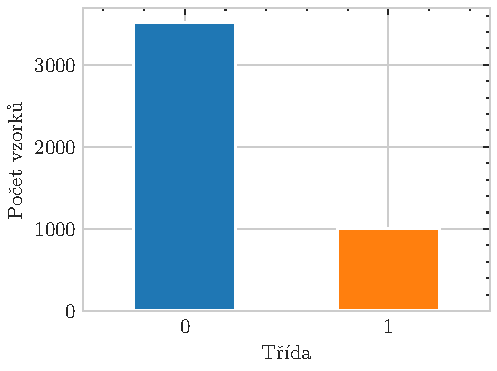
\includegraphics[width=\linewidth]{figures/wesad_labels}
        \caption{Rozdělení datasetu WESAD}
    \end{subfigure}
    \hfill
    \begin{subfigure}[h]{0.48\linewidth}
        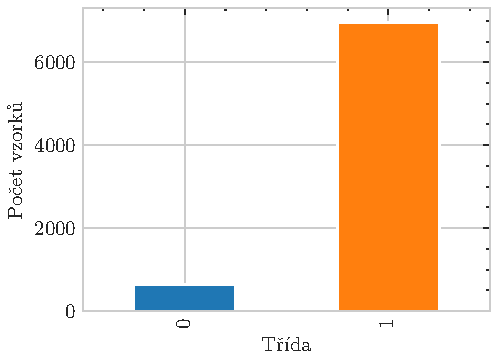
\includegraphics[width=\linewidth]{figures/clas_labels}
        \caption{Rozdělení datasetu CLAS}
    \end{subfigure}
    \caption{Srovnání rozdělení tříd vybraných datasetů. Třída 0 vyjadřuje
    klidový stav a třída 1 vyjadřuje kognitivní zátěž.}
    \label{fig:rozdeleni_trid}
\end{figure}

Během explorace dat byla také zkoumána separovatelnost dat v
nízkodimenzionálních prostorech použitím techniky \gls{UMAP}~\cite{umap2018}
(Uniform Manifold Approximation and Projection) právě pro redukci
dimenzionality. Cílem bylo vizualizovat soubor dat ve formě nižších dimenzí k
získání přehledu o rozdělení tříd a nadhled nad smyslem a rozpoložení dat.
Výsledky této vizualizace je možné vidět na Obr.~\ref{fig:umap}, kde jsou
oranžově vyznačeny body, jež odpovídají kognitivní zátěži.

\begin{figure}[h]
    \begin{subfigure}[h]{0.48\linewidth}
        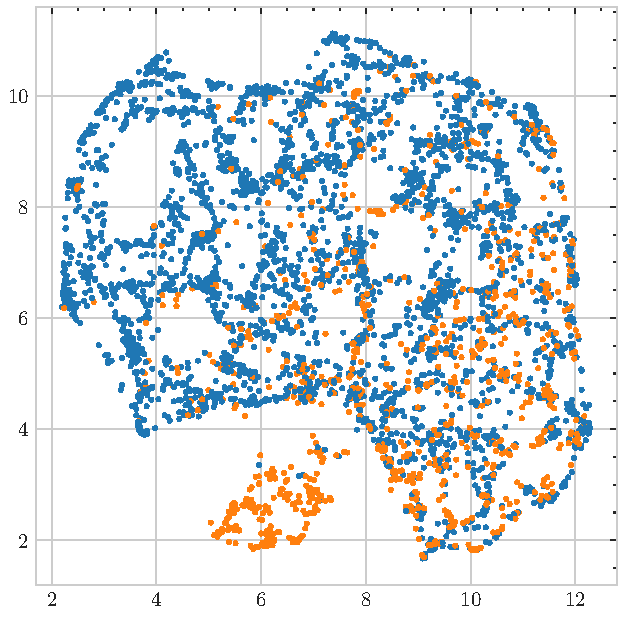
\includegraphics[width=\linewidth]{figures/wesad_umap}
        \caption{WESAD}
    \end{subfigure}
    \hfill
    \begin{subfigure}[h]{0.48\linewidth}
        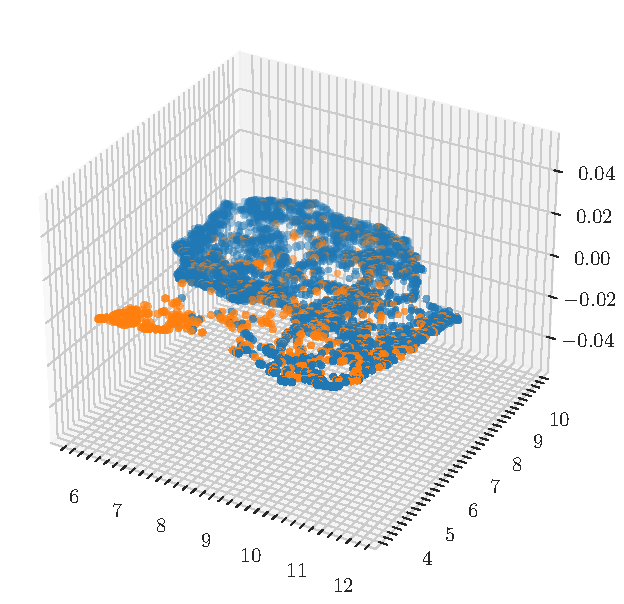
\includegraphics[width=\linewidth]{figures/clas_umap}
        \caption{CLAS}
    \end{subfigure}
    \caption{Vizualizace UMAP projekcí extrahovaných příznaků z datasetu WESAD
    do 2D (vlevo) a 3D latentního prostoru (vpravo). Oranžově třída 1 a modře
    třída 0}
    \label{fig:umap}
\end{figure}

V metodě bylo využito Euklidovské vzdálenostní metriky s hodnotou 0,1 a počtem
sousedních bodů 15. Tyto nízké hodnoty byly zvoleny pro účely zachycení lokální
struktury dat (potenciálně na úkor celkového obrazu), jak ukazuje
Obr.~\ref{fig:umap}. Výsledek 3D projekcí naznačuje potencionální lineární
separovatelnost u malé části souboru. U zbytku souboru by bylo oddělení
pravděpodobně zřetelnější ve vyšších dimenzích a možná nebude lineární. V úvahu
tak přichází strojové učení.